\section{Evaluation}
\label{sec:summary:eval}

In this section, we evaluate the performance of computing a graph summary, as well as its size.
For this evaluation, we use the following:
\begin{itemize}
	\item $G=\left\langle V, A, l_V \right\rangle$ is a graph;
	\item the bisimulation summary of $G$ is $\mathcal{S}_{fbt} = \left\langle \mathcal{W}_{fbt}, \mathcal{B}_{fbt}, l_{\mathcal{W}_{fbt}} \right\rangle$ according to the summarisation relation $R_{fbt}$; and
	\item $\mathcal{S} = \left\langle \mathcal{W}, \mathcal{B}, l_{\mathcal{W}} \right\rangle$ is a summary of $G$ according to the summarisation relation $R$.
\end{itemize}

\subsection{Design}
\label{sec:eval:design}

We describe in this section the design of the evaluation. We first present the environment of our experimental framework. Then, we describe the dimensions of our evaluation.

\subsubsection{Environment}

The bisimulation summary $\mathcal{S}_{fbt}$ is the most precise summary of the data graph, since all incoming and outgoing (and combination of) paths in the summary do exist in the data graph $G$. In this evaluation, we use the forward bisimulation $R_{fb}$ summarisation relation presented in Section~\ref{chap:summary:bisim} as the \emph{gold standard} summary of a data graph. This gold standard summary ensures that all outgoing paths do exist. The presented summarisation relations have been implemented using the Hadoop\footnote{Hadoop: \url{http://hadoop.apache.org/}} MapReduce framework.
% Our Hadoop cluster is composed of 10 machines.

\subsubsection{Evaluation Dimensions}

We present in this section two dimensions we use for evaluating a summary, i.e., the \emph{volume} and the \emph{performance} of the relation.

\begin{quotation}
	\item[\emph{Summary volume.}]
	
	We measure the amount of data from the gold standard summary that is compressed into the evaluated summary. To this end, we compare the volume of the summary against the volume of the gold standard. We report this comparison as the ratio  $\mathcal{S}:\mathcal{S}_{fb}$ of the former to the later.
	
	$$
	\mathcal{S}:\mathcal{S}_{fb} = \frac{\vert \mathcal{W} \vert + \vert \mathcal{B} \vert}{\vert \mathcal{W}_{fb} \vert + \vert \mathcal{B}_{fb} \vert}
	$$
	
	\item[\emph{Algorithm performance.}]
	
	%The MapReduce implementation of the graph summarisation is composed of two separate steps:
	%\begin{inparaenum}[(1)]
	%\item a \emph{mapping} step, where we assign a node of the data graph to its $\sim$-equivalence class; and
	%\item a \emph{edges} step, where we compute the edges of $G^\sim$.
	%\end{inparaenum}
	We evaluate the computational performance of a summarisation relation by analysing the CPU time\footnote{The accumulated CPU time as reported with the \texttt{CPU\_MILLISECONDS} counter of Hadoop.} on the \hyperref[step-he]{Step 3} of the graph summary computation, as described in Section~\ref{chap03:algo:edge-materialisation} for the MapReduce case. We do not report on the performance of the \hyperref[step-hn]{Step 2} because the evaluated summarisation relations have the same complexity, achieving similar times on this step.
\end{quotation}

\subsection{Datasets}
\label{sec:eval:datasets}

We use in this evaluation several datasets of various complexity. We list in the Table~\ref{tab:datasets} the datasets along with some descriptive statistics. The datasets are grouped according to their complexity into four categories, i.e., \emph{Low}, \emph{Medium}, \emph{High}, and \emph{Very High}. We determined the complexity with regards to the volume of a graph and the number of unique types and attributes it possesses.

For each dataset, we present two aspects, i.e., the \emph{schema} and the \emph{structure} of the data graph. With regards to the schema complexity, we report the number of unique edge labels $\vert \mathcal{L}^A \vert$ and the number of unique types $\vert \mathcal{L}^T \vert$ of the data graph. With regards to the structure complexity, we report the size and order of $G$ and  $\mathcal{S}_{fb}$. The order values omit the number of sink nodes, i.e., nodes without outgoing edges which includes literal nodes in the RDF data model.

The $\mathcal{S}_{fb}:G$ column reports the volume ratio of $\mathcal{S}_{fb}$ to $G$ as a percentage, where the volume is the sum of the size and order of a graph. We remark that the volume of the summary $\mathcal{S}_{fb}$ is significantly smaller than the volume of the data graph. This emphasize the performance benefits of using a summary instead of the data graph itself in an application. We note that the bigger the volume ratio, the more complex the data graph is to summarise from a structural point of view. Although the datasets \texttt{bnb} and \texttt{wb} have a similar volume, the volume ratio of the summary on \texttt{bnb} is greater than for \textbf{wb}, i.e., $1.17\%$ to $0.01\%$. This shows that the structure of \texttt{bnb} is more heterogeneous than that of \texttt{wb}.

\begin{table}
	\centering
	\ra{1.2}
	\resizebox{\textwidth}{!}{
		\begin{tabular}{lc@{\hs}rrc@{\hs}rrc@{\hs}rrc@{\hs}r}
			\toprule
			Dataset & \phantom{a} & \multicolumn{2}{c}{Schema} & \phantom{a} & \multicolumn{2}{c}{$G$} & \phantom{a} & \multicolumn{2}{c}{$\mathcal{G}_{fb}$} & \phantom{a} & $\mathcal{G}_{fb}:G$ \\
			\cmidrule{3-4} \cmidrule{6-7} \cmidrule{9-10} \cmidrule{12-12}
			 & \phantom{a} & $\vert \mathcal{L}^T \vert$ & $\vert \mathcal{L}^A \vert$ & \phantom{a} & $\vert V \vert$ & $\vert A \vert$ & \phantom{a} & $\vert \mathcal{V}_{fb} \vert$ & $\vert \mathcal{G}_{fb} \vert$ & \phantom{a} &
			\\
			{\bfseries \underline{Very High}} \\
			\texttt{dbpedia} \cite{dbpedia}
			 & \phantom{a} & \numprint{288524} & \numprint{22369} & \phantom{a} & \numprint{65042837} & \numprint{233051608} & \phantom{a} & \numprint{6884121} & \numprint{33990765} & \phantom{a} & 13.71\% \\
			\midrule
			{\bfseries \underline{High}} \\
			\texttt{twc-logd} \cite{twc-logd}
			 & \phantom{a} & 450 & \numprint{10060} & \phantom{a} & \numprint{3398947} & \numprint{67505792} & \phantom{a} & \numprint{5565} & \numprint{121873} & \phantom{a} & 0.18\% \\
			\texttt{enipedia} \cite{enipedia}
			 & \phantom{a} & 128 & 267 & \phantom{a} & \numprint{413520} & \numprint{4463566} & \phantom{a} & 1037 & \numprint{21419} & \phantom{a} & 0.46\% \\
			\midrule
			{\bfseries \underline{Medium}} \\
			\texttt{b3kat} \cite{b3kat}
			 & \phantom{a} & 20 & 30 & \phantom{a} & \numprint{85795956} & \numprint{592778746} & \phantom{a} & \numprint{782056} & \numprint{3230936} & \phantom{a} & 0.59\% \\
			\texttt{ecs} \cite{ecs}
			 & \phantom{a} & 24 & 120 & \phantom{a} & \numprint{167390} & \numprint{955112} & \phantom{a} & \numprint{8232} & \numprint{51494} & \phantom{a} & 5.32\% \\
			\texttt{lobid} \cite{lobid-resources}
			 & \phantom{a} & 19 & 46 & \phantom{a} & \numprint{124691274} & \numprint{625941644} & \phantom{a} & \numprint{51529} & \numprint{746099} & \phantom{a} & 0.11\% \\
			\texttt{bnb} \cite{bnb}
			 & \phantom{a} & 27 & 53 & \phantom{a} & \numprint{12246306} & \numprint{89733453} & \phantom{a} & \numprint{146956} & \numprint{1046714} & \phantom{a} & 1.17\% \\
			\texttt{datos} \cite{datos}
			 & \phantom{a} & 23 & 143 & \phantom{a} & \numprint{7412312} & \numprint{58048932} & \phantom{a} & \numprint{360822} & \numprint{2504262} & \phantom{a} & 4.38\% \\
			\texttt{gnd} \cite{gnd}
			 & \phantom{a} & 22 & 35 & \phantom{a} & \numprint{962930} & \numprint{7940373} & \phantom{a} & \numprint{9664} & \numprint{88875} & \phantom{a} & 1.11\% \\
			\texttt{eures} \cite{eures}
			 & \phantom{a} & 18 & 49 & \phantom{a} & \numprint{288862} & \numprint{4146421} & \phantom{a} & \numprint{2205} & \numprint{37052} & \phantom{a} & 0.89\% \\
			\midrule
			{\bfseries \underline{Low}} \\
			\texttt{europeana} \cite{europeana}
			 & \phantom{a} & 5 & 58 & \phantom{a} & \numprint{5559452} & \numprint{40773834} & \phantom{a} & \numprint{4792} & \numprint{72125} & \phantom{a} &  0.17\% \\
			\texttt{wb} \cite{wb}
			 & \phantom{a} & 4 & 174 & \phantom{a} & \numprint{11210832} & \numprint{84345613} & \phantom{a} & 293 & \numprint{6987} & \phantom{a} & 0.01\% \\
			\texttt{cordis} \cite{cordis}
			 & \phantom{a} & 7 & 63 & \phantom{a} & \numprint{729780} & \numprint{7101623} & \phantom{a} & \numprint{2245} & \numprint{36783} & \phantom{a} & 0.50\% \\
			\texttt{ny-times} \cite{ny-times}
			 & \phantom{a} & 2 & 38 & \phantom{a} & \numprint{22662} & \numprint{345888} & \phantom{a} & 65 & 794 & \phantom{a} & 0.23\% \\
			\bottomrule
		\end{tabular}
	}
	\caption{Descriptive statistics of the datasets. The Schema column reports the number in $G$ of unique edges labels $\vert \mathcal{L}^A \vert$ and of unique types $\vert \mathcal{L}^T \vert$. The column $G$ reports the order and the size of the data graph. The column $\mathcal{G}_{fb}$ reports the order and the size of the summary $\mathcal{G}_{fb}$ of the graph $G$. The $\mathcal{G}_{fb}:G$ column reports as a percentage the volume ratio of $\mathcal{G}_{fb}$ to $G$.}
	\label{tab:datasets}
\end{table}

\subsection{Results}

We evaluate and compare in this section the different graph summary algorithm according to the volume and the computational complexity.
We note the mean of measurements in a category as $\mu_{L}$, $\mu_{M}$, $\mu_{H}$, and $\mu_{VH}$, respectively.

\subsubsection{Graph Summary Volume}

The Table~\ref{tab:volume-ratio} reports the volume ratio between the summary $\mathcal{S}$ and the gold standard summary $\mathcal{S}_{fb}$. We report also the mean $\mu$ for each category of datasets complexity.

The summaries based only on the type information, i.e., $R_{st}$ and $R_t$, exhibit a higher compression compared to the gold standard. With regards to the gold standard volume, the volume ratio is under $5\%$ on the \emph{Low} and \emph{Medium} datasets and at most half on the more complex datasets. On average, we note that the volume of a summary with $R_{st}$ is slightly higher than with $R_t$. The reason is that a node of the data graph can be mapped to several sumnodes with the \emph{Single-Type} summary $R_{st}$, which leads to an increase of the size of the summary.

The attribute feature appears to be a better feature for summarising a graph than type. Indeed, the volume ratio of $\mathcal{S}_a$ and $\mathcal{S}_{ioa}$ remains stable with \emph{Medium} ($42.51$ and $51.45$, resp.) and \emph{High} ($47.99$ and $66.13$, resp.) datasets. However, this is not the case with the $\mathcal{S}_{st}$ and $\mathcal{S}_t$ summaries. 

We can observe a correlation between the volume ratio and the size of $\mathcal{L}^T$.
We note that the \emph{Attributes} summarisation $R_a$ actually achieves the lowest ratio on the \texttt{dbpedia} dataset. This shows that the use of attributes in \texttt{dbpedia} is homogeneous across types. The volume ratio of the \emph{IO Attributes} summary $\mathcal{S}_{ioa}$ is on average on par with the ratio of the \emph{Attributes} summary $\mathcal{S}_a$, indicating a certain homogeneity of incoming edges in the data graph.

By using both type and attribute information as with the \emph{Attributes \& Types} summarisation relation $R_{at}$, we remark that this can lead to a significant increase of the summary volume. Indeed, the combination of the features on \texttt{b3kat} and \texttt{lobid} exhibits a much higher ratio than when taken separately, e.g., $55.87$ and $84.06$ respectively with $\mathcal{S}_{at}$, against $27.43$ and $49.83$ with $\mathcal{S}_a$. We can conclude that a sparse usage of attributes with a type creates an explosion of combinations. In general, the type feature is less stable than the attribute feature.

\begin{figure}
	\centering
	\resizebox{\textwidth}{!}{
		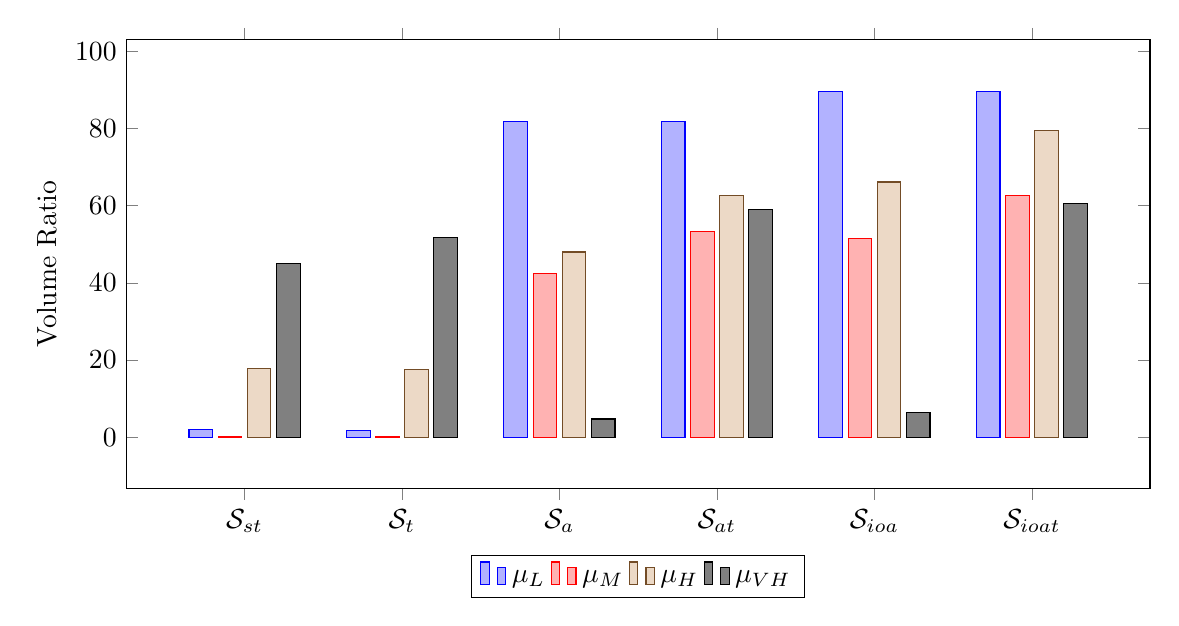
\begin{tikzpicture}
		\begin{axis}[
		ybar,
		symbolic x coords={$\mathcal{S}_{st}$,$\mathcal{S}_{t}$,$\mathcal{S}_{a}$,$\mathcal{S}_{at}$,$\mathcal{S}_{ioa}$,$\mathcal{S}_{ioat}$},
		enlargelimits=0.15,
		ylabel={Volume Ratio},
		x=2cm,
		bar width=0.3cm,
		xtick=data,
		legend style={at={(0.5,-0.15)},
			anchor=north,legend columns=-1},
		]
		\addplot coordinates {
			($\mathcal{S}_{st}$,1.89)
			($\mathcal{S}_{t}$,1.77)
			($\mathcal{S}_{a}$,81.73)
			($\mathcal{S}_{at}$,81.74)
			($\mathcal{S}_{ioa}$,89.57)
			($\mathcal{S}_{ioat}$,89.57)
		};
		
		\addplot coordinates {
			($\mathcal{S}_{st}$,0.23)
			($\mathcal{S}_{t}$,0.22)
			($\mathcal{S}_{a}$,42.51)
			($\mathcal{S}_{at}$,53.37)
			($\mathcal{S}_{ioa}$,51.45)
			($\mathcal{S}_{ioat}$,62.68)
		};
		
		\addplot coordinates {
			($\mathcal{S}_{st}$, 17.81)
			($\mathcal{S}_{t}$,17.60)
			($\mathcal{S}_{a}$,47.99)
			($\mathcal{S}_{at}$,62.55)
			($\mathcal{S}_{ioa}$,66.13)
			($\mathcal{S}_{ioat}$,79.45)
		};

		\addplot coordinates {
			($\mathcal{S}_{st}$, 45.00)
			($\mathcal{S}_{t}$,51.81)
			($\mathcal{S}_{a}$,4.71)
			($\mathcal{S}_{at}$,59.10)
			($\mathcal{S}_{ioa}$,6.41)
			($\mathcal{S}_{ioat}$,60.56)
		};
		\legend{$\mu_L$,$\mu_M$,$\mu_H$,$\mu_{VH}$}
		\end{axis}
		\end{tikzpicture}
	}
	\caption{Volume ratio of the graph summaries}
	\label{fig:vol-ration-bar}
\end{figure}

\subsubsection{Performance of the Summarisation Relation}

The Table~\ref{tab:cpu-time} reports the CPU time in $ms$ of the \emph{edges} step in the graph summarisation computation. The reported times are the average of two runs of an algorithm for a certain dataset.

The $R_{st}$ and $R_t$ summarisation relations may have undefined mappings due to missing type statements for some entities. For performance reason, the node $\mathfrak{U}$ are filtered from the resulting summary. Therefore, reported run times in Table~\ref{tab:cpu-time} from $R_{st}$ and $R_t$ cannot be compared to others.

On the \emph{Medium}, \emph{High}, and \emph{Very High} datasets, the time taken by the $R_{st}$ summarisation on the \hyperref[step-he]{Step 3} of the graph summary computation is higher than $R_t$. This highlights the property of the $R_{st}$ summarisation of being a many-to-many binary relation. As a consequence, we need to compute all the possible combinations of edges between the sumnodes.
We note that the incoming attribute feature in $R_{ioa}$ and $R_{ioat}$ does not imply a higher runtime when compared to $R_{a}$ and $R_{at}$.

\begin{figure}
	\centering
	\resizebox{\textwidth}{!}{
		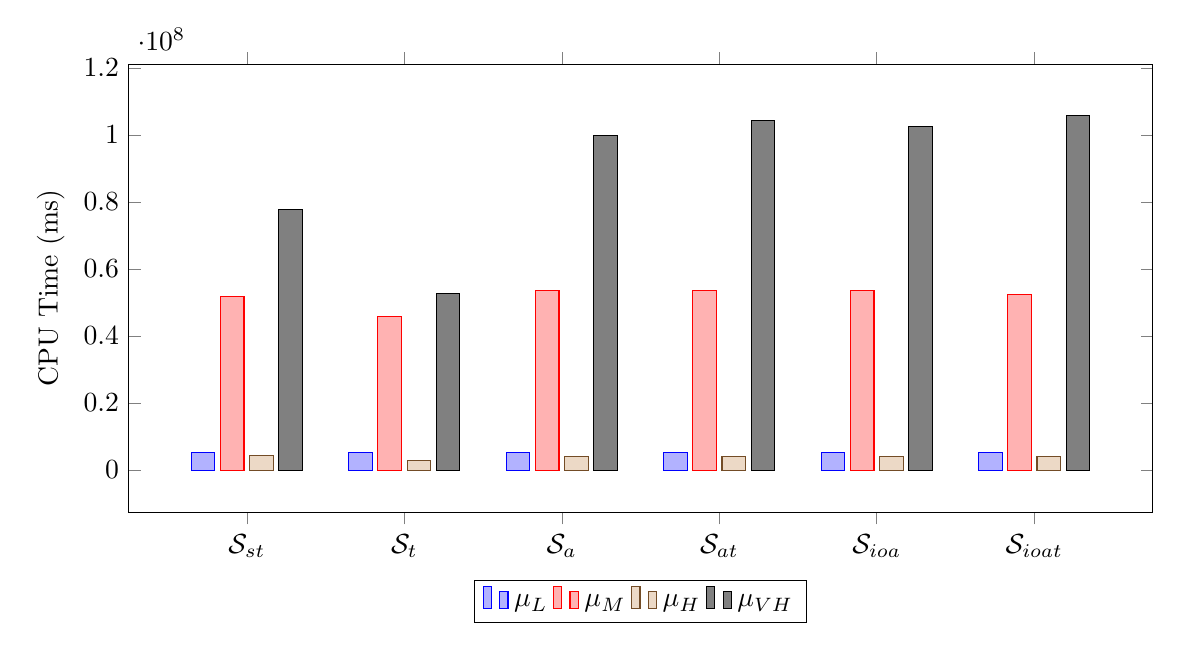
\begin{tikzpicture}
		\begin{axis}[
		ybar,
		symbolic x coords={$\mathcal{S}_{st}$,$\mathcal{S}_{t}$,$\mathcal{S}_{a}$,$\mathcal{S}_{at}$,$\mathcal{S}_{ioa}$,$\mathcal{S}_{ioat}$},
		enlargelimits=0.15,
		ylabel={CPU Time (ms)},
		x=2cm,
		bar width=0.3cm,
		xtick=data,
		legend style={at={(0.5,-0.15)},
			anchor=north,legend columns=-1},
		]
		\addplot coordinates {
			($\mathcal{S}_{st}$, 5181727)
			($\mathcal{S}_{t}$, 5140988)
			($\mathcal{S}_{a}$, 5208950)
			($\mathcal{S}_{at}$, 5227250)
			($\mathcal{S}_{ioa}$, 5254718)
			($\mathcal{S}_{ioat}$, 5212401)
		};
		
		\addplot coordinates {
			($\mathcal{S}_{st}$, 51724125)
			($\mathcal{S}_{t}$, 45942442)
			($\mathcal{S}_{a}$, 53505035)
			($\mathcal{S}_{at}$, 53487935)
			($\mathcal{S}_{ioa}$, 53557640)
			($\mathcal{S}_{ioat}$, 52440249)
		};
		
		\addplot coordinates {
			($\mathcal{S}_{st}$, 4246345)
			($\mathcal{S}_{t}$, 2763572)
			($\mathcal{S}_{a}$, 3962202)
			($\mathcal{S}_{at}$, 3942577)
			($\mathcal{S}_{ioa}$, 3989825)
			($\mathcal{S}_{ioat}$, 4032795)
		};

		\addplot coordinates {
			($\mathcal{S}_{st}$, 77643685)
			($\mathcal{S}_{t}$, 52608760)
			($\mathcal{S}_{a}$, 99839325)
			($\mathcal{S}_{at}$, 104255540)
			($\mathcal{S}_{ioa}$, 102540080)
			($\mathcal{S}_{ioat}$, 105685365)
		};
		
		\legend{$\mu_L$,$\mu_M$,$\mu_H$,$\mu_{VH}$}
		\end{axis}
		\end{tikzpicture}
	}
	\caption{Performance comparison of the graph summaries}
	\label{fig:cpu-time-bar}
\end{figure}
